\documentclass[../main.tex]{subfiles}
\graphicspath{{img},{img/ink},{ink}}

\begin{document}

\begin{tcolorbox}[
    width=\textwidth,
    height=\textheight,
    title=Versuch: Auf- und Entlandekurve eines Kodensators,
    fonttitle=\Large,
    before title=\vspace{0.2cm}, after title=\vspace{0.2cm},
    colback=white,
    title filled=true, 
    colbacktitle=mygray,
    colframe=black,
    coltitle=black,
]
    
    \vspace{0.2cm}
\textbf{Klassenstufe}: 9/10

    \vspace{0.4cm}
    
    \textbf{Fachlicher Bezug}: Kondensator, Zeitkonstante, Spannungs- und Strommessung 
    
    \vspace{0.4cm}
    
    \textbf{Material}: Mobile-CASSY + 2 Sensorstecker, iPad + CASSY-App, Netzgerät 30 V, Kondensator $C=0.1 \, \text{F}$, Widerstand $R = 47 \, \Omega$, Schalter, Experimentierkabel

    \vspace{0.5cm}
        \begin{minipage}[c]{0.5\textwidth}
            \centering
            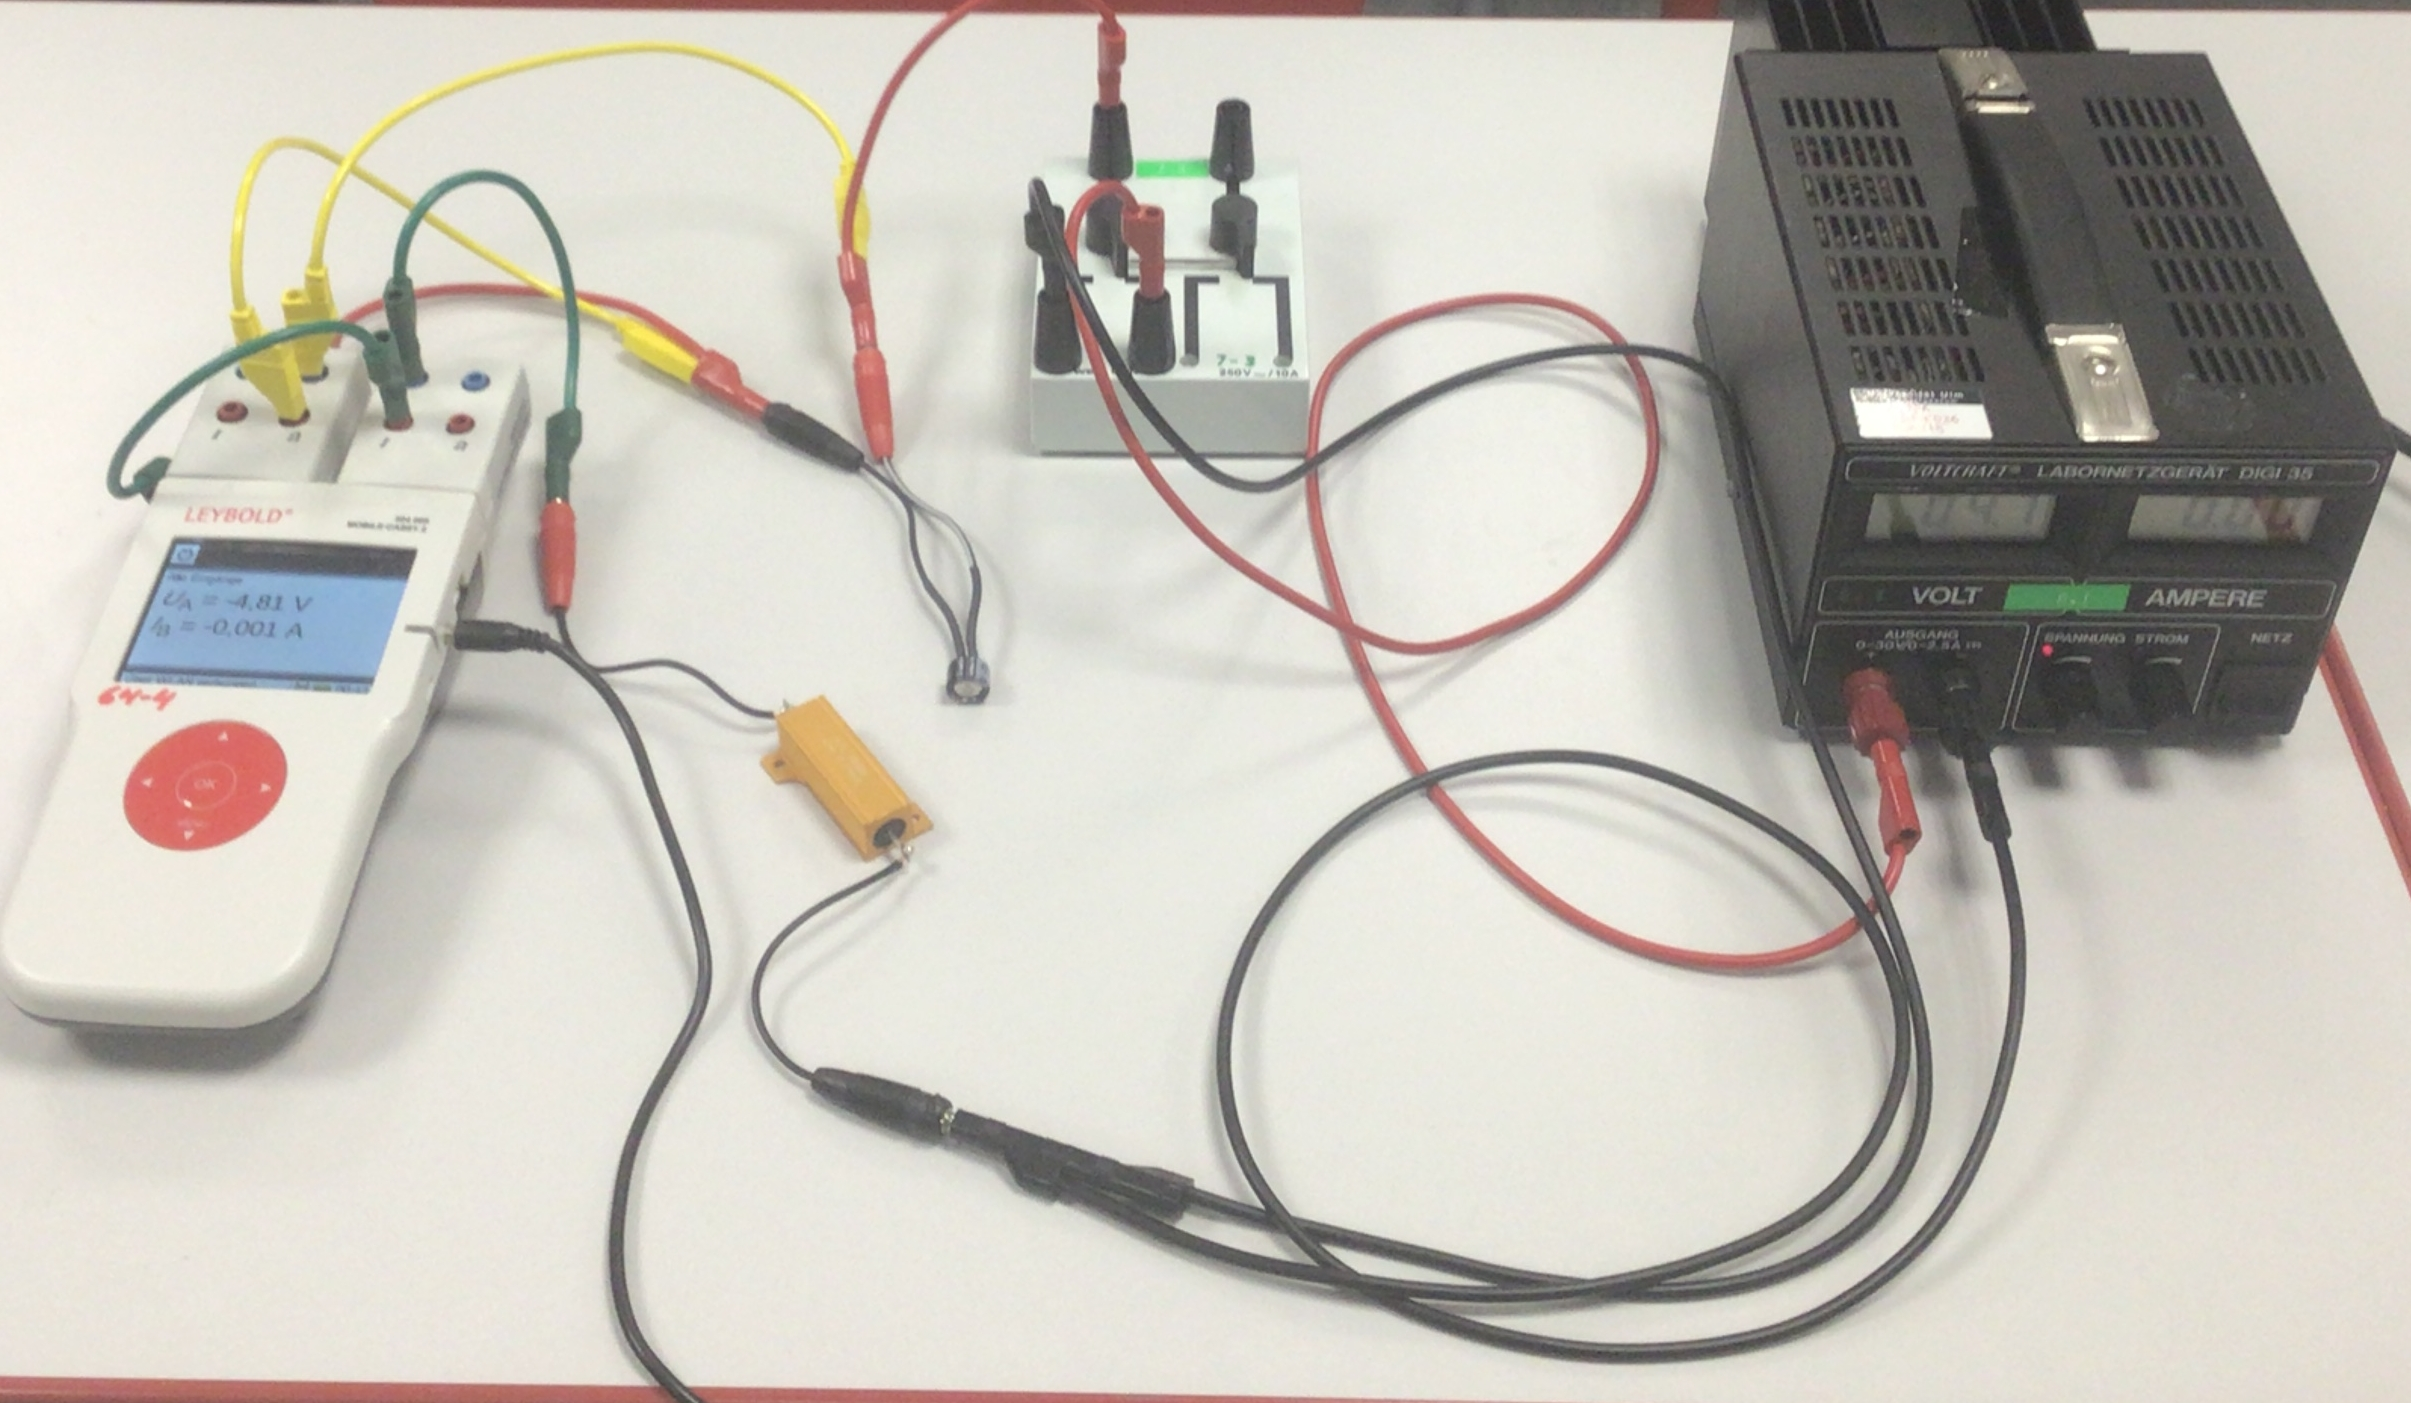
\includegraphics[width=0.85\textwidth]{img/versuchsaufbau}
        \end{minipage}
        \begin{minipage}[c]{0.5\textwidth}
            \vspace{-0.3cm}
            \begin{center}
                \begin{circuitikz} 
                \ctikzset{
                    bipoles/capacitor/width/.initial=.1,
                    european resistors
                }
                \draw   (0,0) node[spdt] (s) {}
                % middle part
                (s.in) to [short] (-1,0) coordinate (cr)
                %(cr) node[circ] {}
                (cr) to [C, l_={$C$}] (-2,0) coordinate (cl)
                %(cl) node[circ] {}
                % voltage measurement
                (cr) to [short] (-1,-1.4) coordinate (voltmeter_right)
                (cl) to [short] (-2,-1.4) coordinate (voltmeter_left)
                (voltmeter_left) to [voltmeter] (voltmeter_right)
                % current measurement
                (cl) to [R={$R$}] (-4,0) coordinate (rl)
                (rl) to [ammeter,mirror,invert] (-5.5,0) coordinate (al)
                %bottom part
                (al) to [short] (-5.5,-2) coordinate (al_down)
                (s.out 2) to [short] (s.out 2|-0,-2) coordinate (s_out_2_down)
                (s_out_2_down) to [short] (al_down)
                %top part
                (al) to [short] (-5.5,1.5) coordinate (al_up)
                (s.out 1) to [short] (s.out 1|-0,1.5) coordinate (s_out_1_up)
                (s_out_1_up) to [battery1, xshift=-5mm] (al_up)
                ;
                \node at (-2.3,1.9) {$U$};
                \draw (al_down) ++ (0,0.3) node[ground]{}; 
            \end{circuitikz}
            \end{center}
            
        \end{minipage}
    
    \vspace{0.4cm}
    \textbf{Aufbau}: Das Experiment besteht aus Lade- und Entladestromkreis. Ein Schalter ermöglicht einen Wechsel. Steckplätze am Mobile-CASSY messen die Stromstärke und die Spannung. Die Messung der Stromstärke (in Reihe) muss im Lade- und Entladestromkreis möglich sein. Die Spannungsmessung erfolgt parallel zum Kondensator. Das Mobile-CASSY stellt einen Wlan-Access-Point zur Verfügung. Um eine Verbindung mit dem iPad herzustellen, verbindet man sich mit dem Access-Point und startet die CASSY-App. 
    
    \vspace{0.4cm} 
    \begin{minipage}[]{0.75\textwidth}
        \textbf{Durchführung}: Zu Beginn des Versuchs speichert der Kondensator keine Spannung. Der Entladestromkreis ist geschlossen. Für den Ladestromkreis wird nun eine Spannung von ca. $U=5$ V bereitgestellt. Anschließend wird die Messwertaufnahme in der CASSY-App gestartet. Lade-und Entladevorgang werden aufgezeichnet. 

        \vspace{0.4cm}
    \textbf{Ergebnis}: Man erhält die dargestellten Lade-und Entladekurven. Die schwarze Kurve entspricht dabei der gespeicherten Spannung im Kondensator. Die rote Kurve zeigt die Stromstärke.
    \end{minipage}
    \begin{minipage}[]{0.24\textwidth}
        \vspace{-0.2cm}
        \begin{center}
            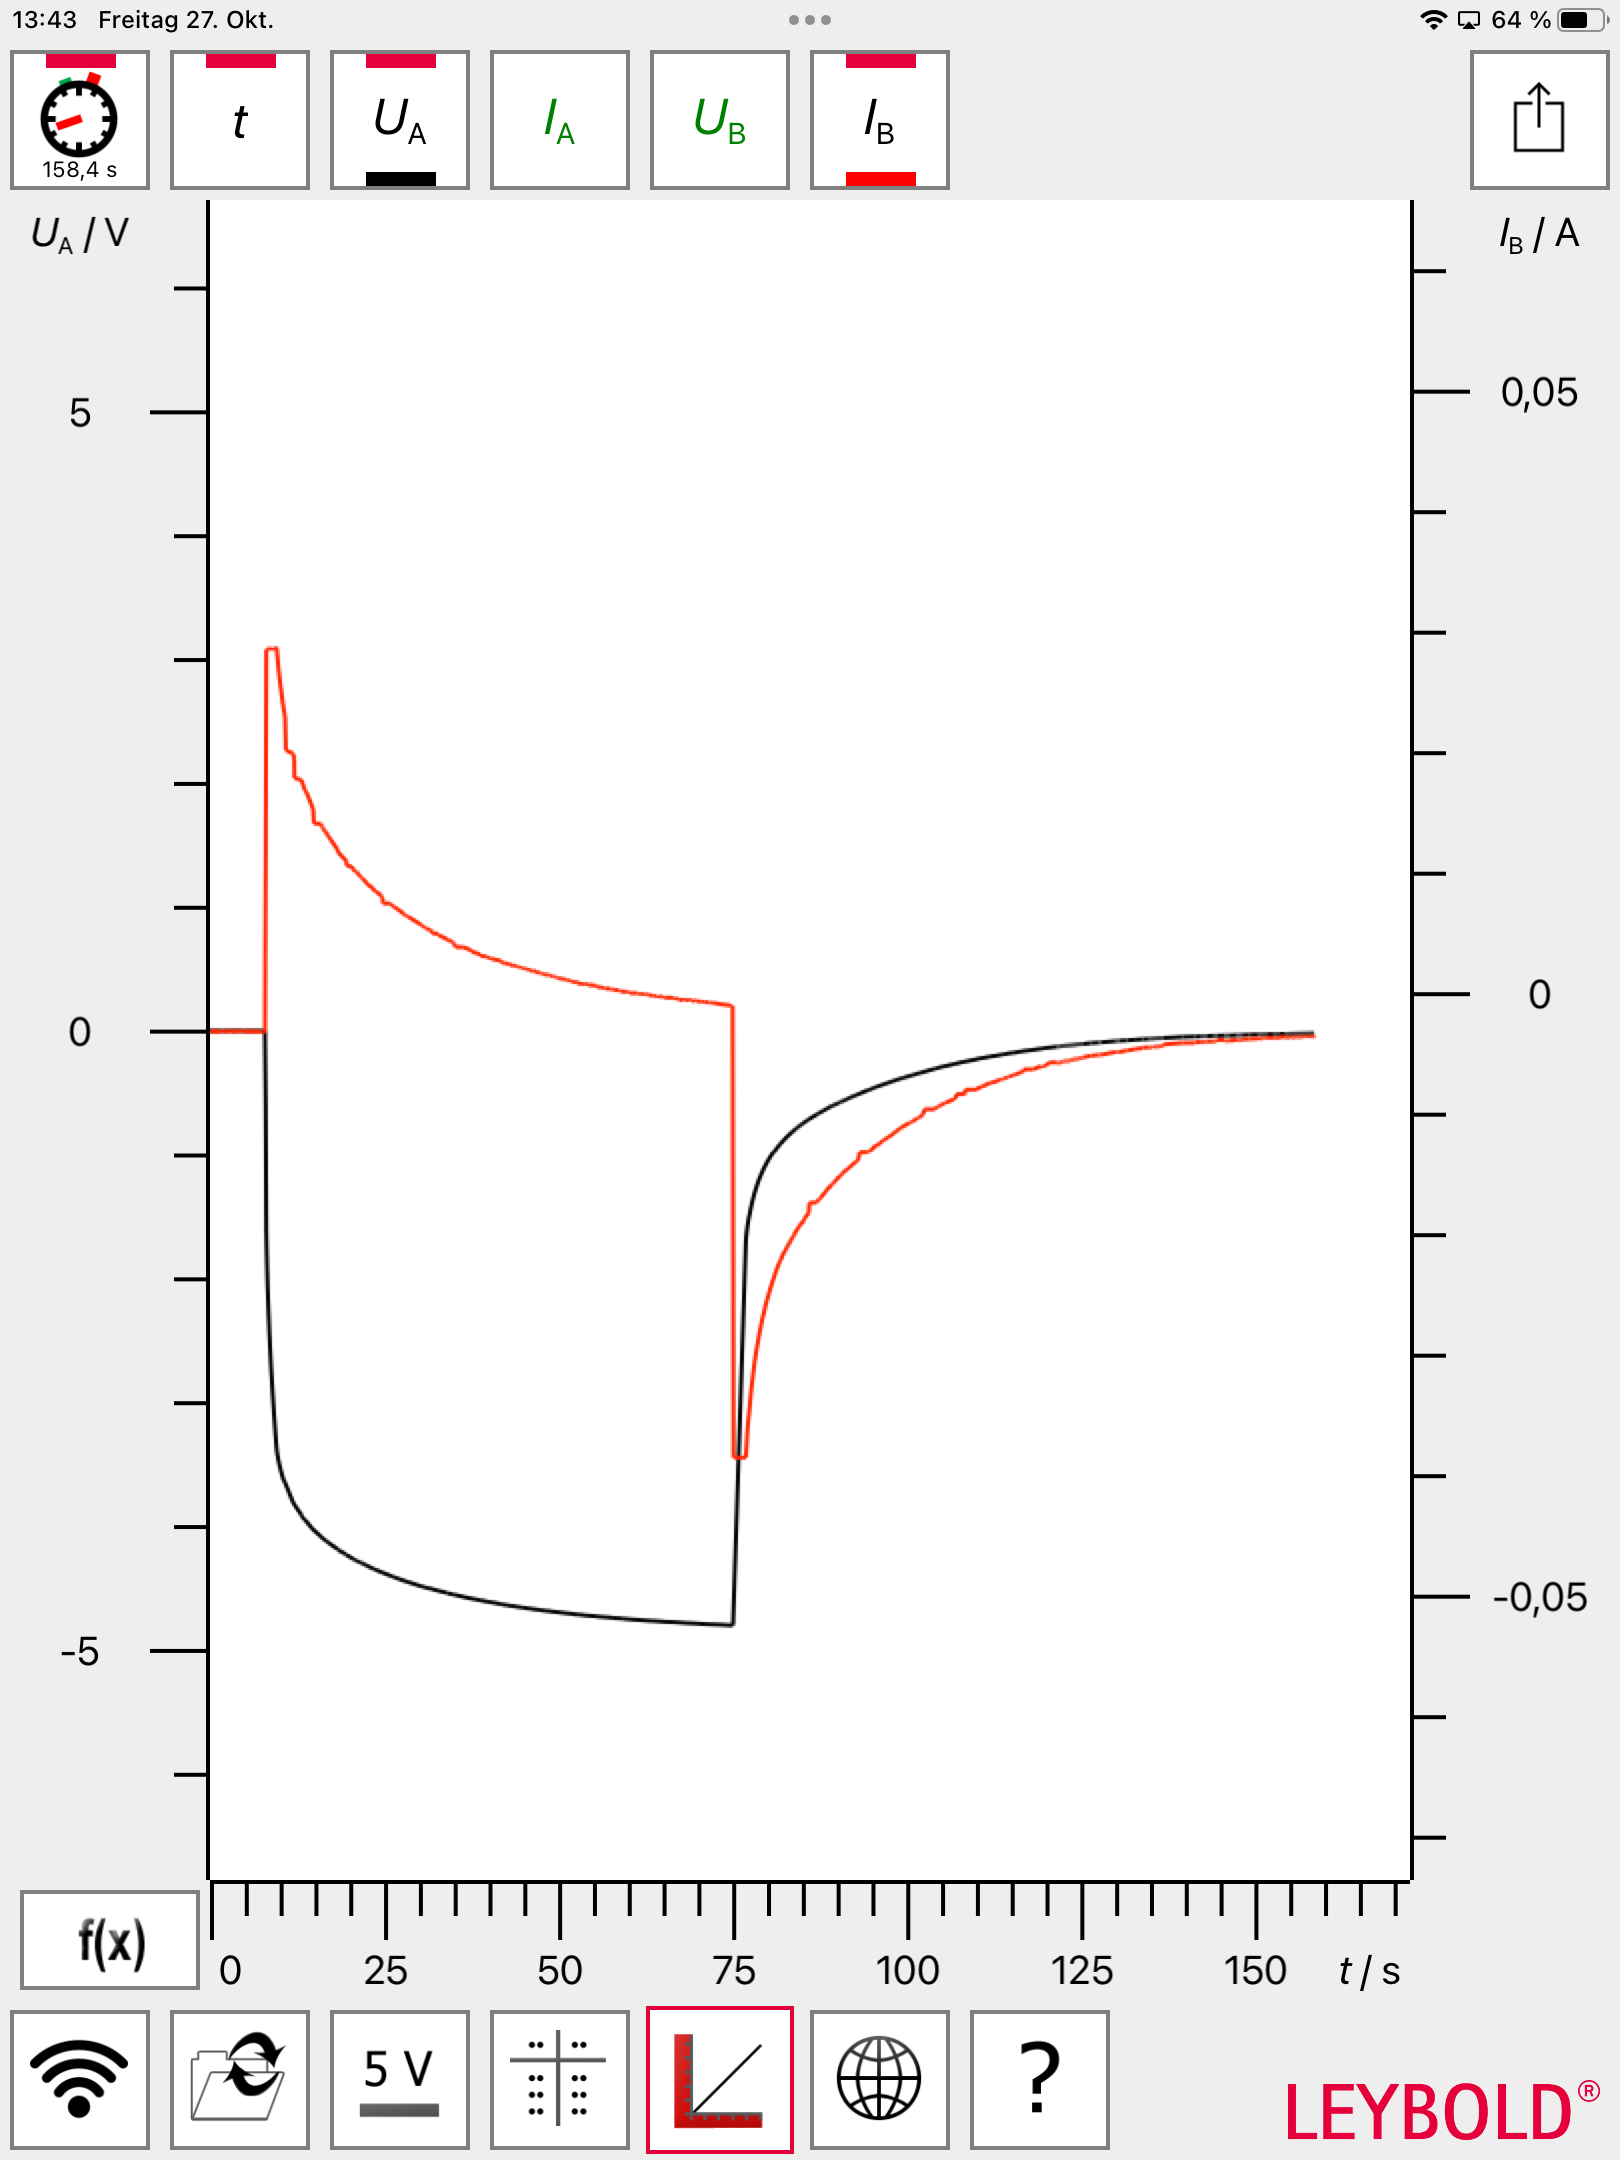
\includegraphics[width=0.85\textwidth]{img/cassy}
        \end{center}
    \end{minipage}
  
    \vspace{0.4cm}
    \textbf{Didaktische Bemerkungen}: Beim Entladevorgang wird eine Umkehr in der Stromrichtung beobachtet. Vor Versuchsbeginn können dazu Hypothesen aufgestellt werden. Die gespeicherte Spannung des geladenen Kondensators führt beim Entladen zu einer Umkehr der ursprünglichen Stromrichtung. Das Aufladen wird deshalb als \glqq negative Spannung\grqq{} aufgetragen. Um Verwirrungen zu vermeiden, sollte hier aber eine ausführliche Diskussion über den Bezugspunkt (Masse) bei der Spannungsmessung erfolgen.     
    
    \vspace{0.4cm}
    \textbf{Bemerkungen}: Die Zeitkonstante $\tau=R \cdot C$ liefert die Zeit, nach der die Spannung (bzw. Stromstärke) um einen Faktor von ca. $1/3$ gefallen ist. \\
    Um eine möglichst hohe Abtastrate der Sensorstecker zu erreichen, ist es sinnvoll Spannung-und Strommessung getrennt, an zwei verschiedenen Steckplätzen, vorzunehmen.\\
Bei Verwendung der CASSY-App kann es zu Schwierigkeiten bei der Positionierung des Koordinatensystems kommen. Hier hilft in der Regel ein kurzer Wechsel der Steckplätze.
\end{tcolorbox}


\end{document}
